\section{Results (\textit{Jacob Salomonsen})}

\subsection{Running time}
After running the test described in \autoref{sec:testing} on both the CPU- and the GPU-version
\insfig{./images/result.png}{1.0\textwidth}{results}{results}


\subsection{Other characteristics}

\begin{figure}[H]
\centering
\subfigure[tunnel]{
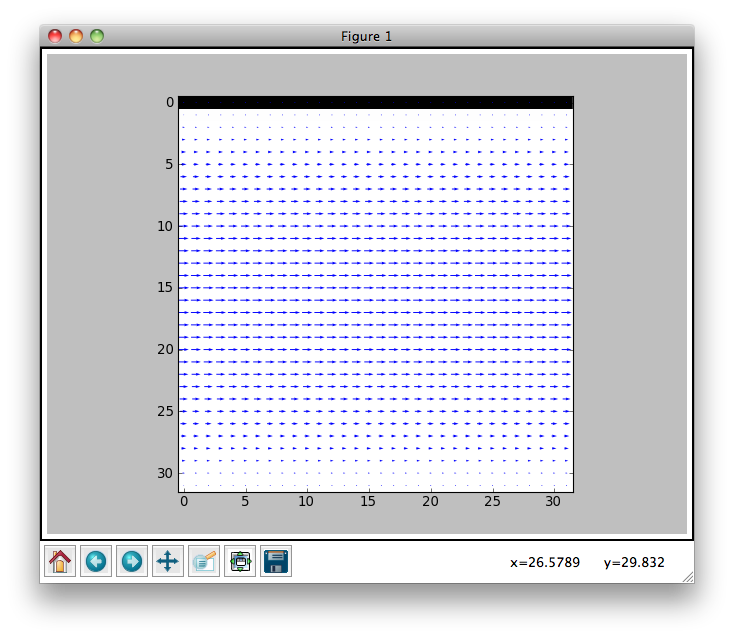
\includegraphics[width=0.47\textwidth]{./images/cuda_tunnel_32_32_900.png}
\label{tunnel}
}
\hspace{1pt}
\subfigure[tunnelcolor]{
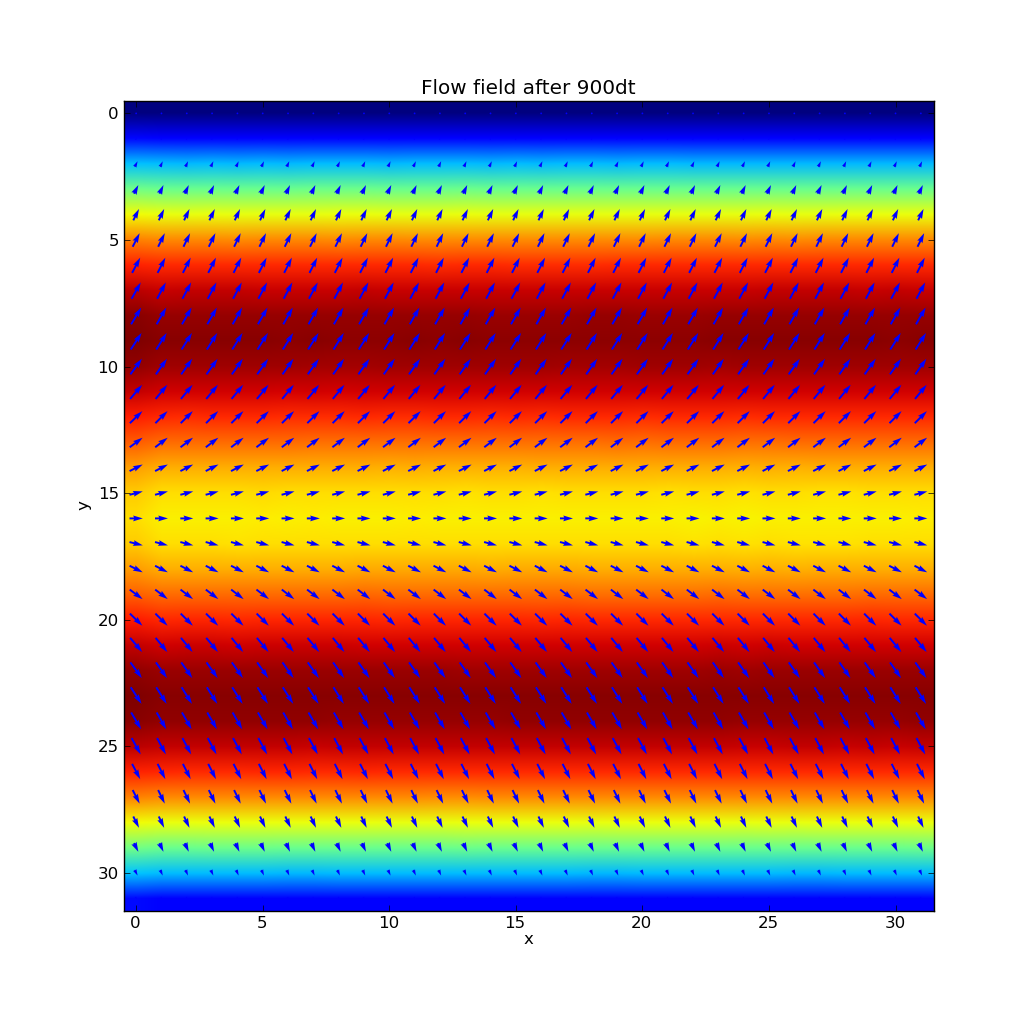
\includegraphics[width=0.47\textwidth]{./images/cuda_tunnel_32_32_900_color.png}
\label{tunnelcolor}
}
\caption{Testing that the three implementations produces the same output under equal conditions}
\label{tunnelimages}
\end{figure}



\begin{figure}[H]
\centering
\subfigure[lid]{
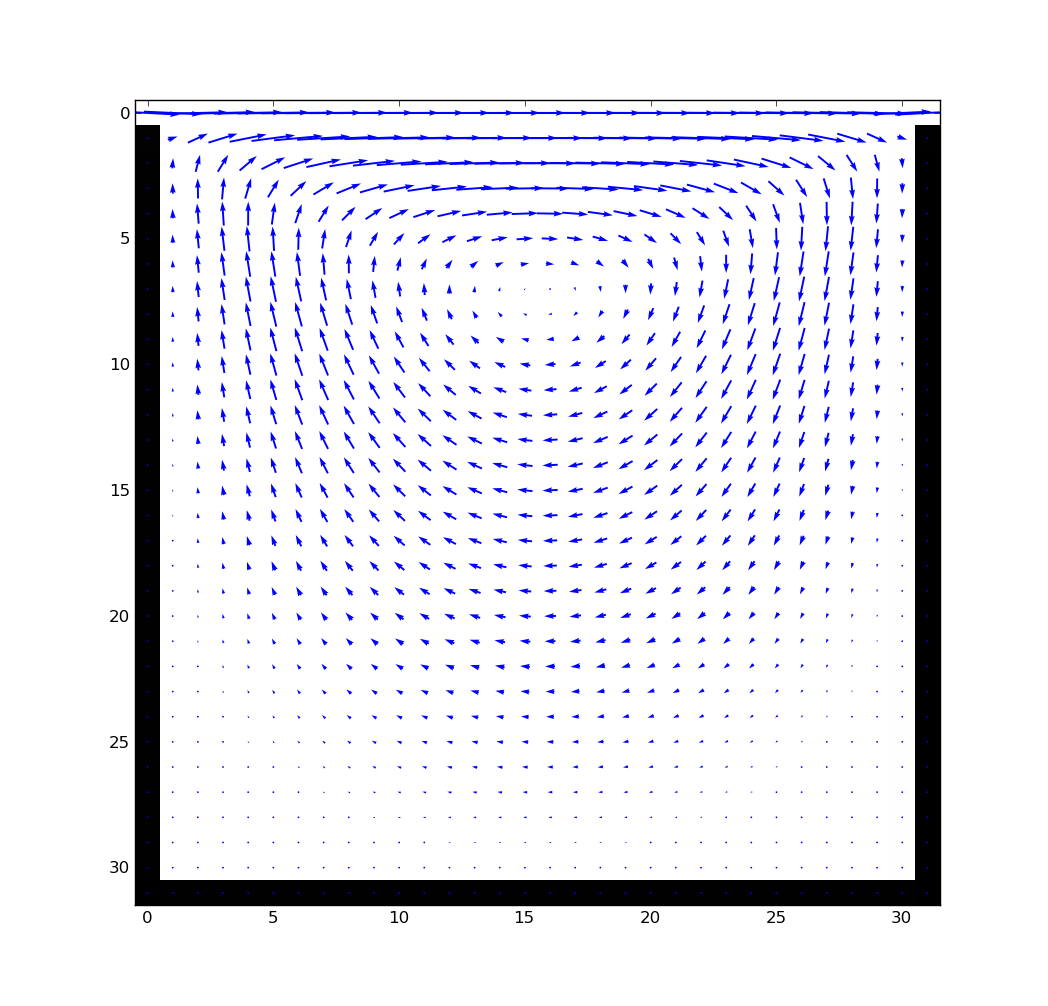
\includegraphics[width=0.47\textwidth]{./images/cuda_lid_32_32_900.png}
\label{lid}
}
\hspace{1pt}
\subfigure[lidcolor]{
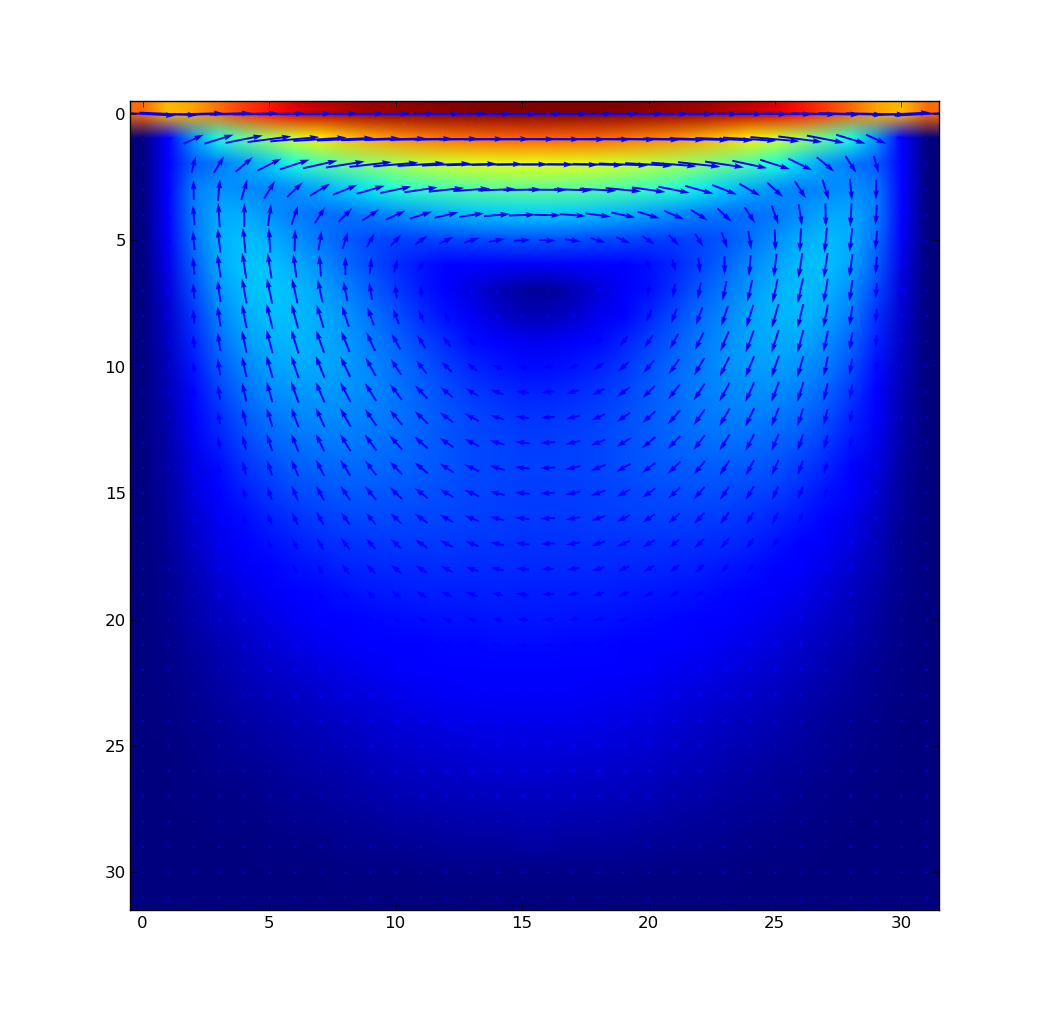
\includegraphics[width=0.47\textwidth]{./images/cuda_lid_32_32_900_color.png}
\label{lidcolor}
}

\subfigure[lidhighit]{
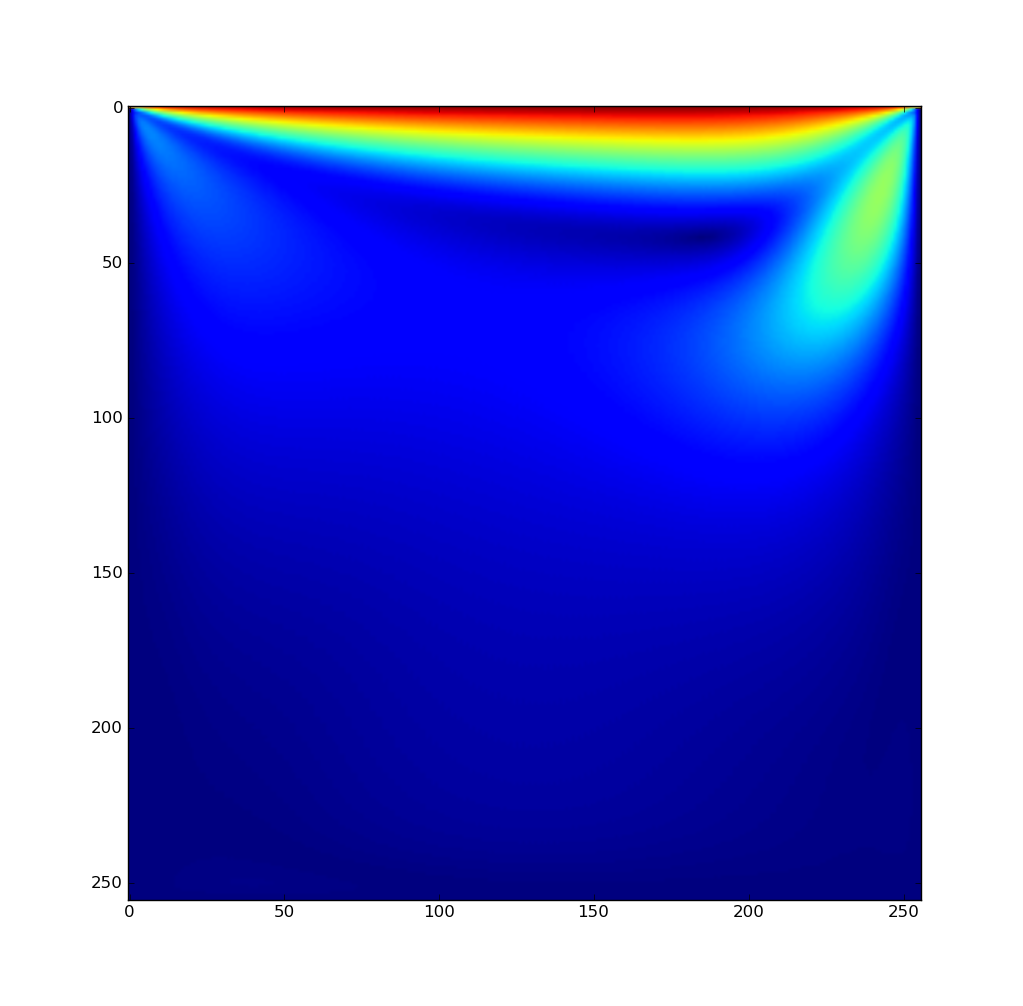
\includegraphics[width=0.47\textwidth]{./images/cuda_lid_256_256_2700.png}
\label{lidhighit}
}
\hspace{1pt}
\subfigure[lidref]{
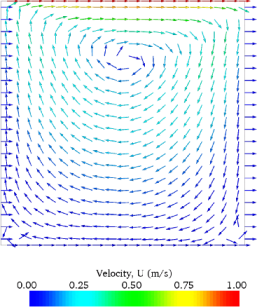
\includegraphics[width=0.35\textwidth]{./images/lidref.png}
\label{lidref}
}
\caption{}
\label{lidimages}
\end{figure}


